\documentclass[a4paper]{article}
\usepackage[T1]{fontenc}
\usepackage[utf8]{inputenc}
\usepackage{lmodern}
\usepackage{amsmath,amssymb}
\usepackage[top=3cm,bottom=2cm,left=2cm,right=2cm]{geometry}
\usepackage{fancyhdr}
\usepackage{esvect}
\usepackage{xcolor}
\usepackage{tikz}\usetikzlibrary{calc}

\parskip 1em\parindent 0pt

\begin{document}

\pagestyle{fancy}
\fancyhf{}
\setlength{\headheight}{15pt}
\fancyhead[L]{Electromagnétisme}\fancyhead[R]{Question 48}

% Énoncé
\begin{center}
	\large{\boldmath{\textbf{Modèle de Drude}}}
\end{center}

% Correction

Un métal est un conducteur qui contient un grand nombre d'électrons libres. Soit $n_e$ la densité d'électrons libres du métal considéré. On utilise le modèle de Drude qui permet d'analyser le mouvement de ces électrons libres.\\
Selon ce modèle, un électron libre est soumis à une force de viscosité $\vv f=-m \dfrac{\vv v}{\tau}$ où $\tau$ est la durée moyenne entre deux chocs de l'électron avec le réseau cristallin supposé immobile. Typiquement, $\tau\simeq 10^{-14}$ s.\par
PDF sur un électron libre : $m\dfrac{\partial \vv*ve}{\partial t}=-e\vv E- \dfrac{m}{\tau}\vv*ve$\\
En notation opticienne, $-mi\omega \underline{\vv*ve}=-e \underline{\vv E}- \dfrac{m}{\tau}\underline{\vv*ve}$ donc $\underline{\vv*ve}=\dfrac{-e\vv E}{m \left( \dfrac{1}{\tau}-i\omega \right)}=\dfrac{-\tau e\vv E}{m(1-i\omega\tau)}$\\
Donc $\underline{\vv j}=-n_ee \underline{\vv*ve}=\dfrac{n_ee^2\tau}{m}\dfrac{1}{1-i\omega\tau}\underline{\vv E}$ donc
\begin{center}
\fcolorbox{red}{white}{\(\gamma=\dfrac{n_ee^2\tau}{m}\dfrac{1}{1-i\omega\tau}\)}
\end{center}

\underline{1$^{\mathrm{er}}$ cas :} domaine radio, $f<10^{11}$ Hz ($\omega<10^{12}$ rad/s)\\
Alors $\omega\tau<10^{-2}$ et le métal a une conductivité réelle : $\gamma\simeq\dfrac{n_ee^2\tau}{m}$\\
Amortissement de l'onde : le métal absorbe complètement l'onde au bout de quelques longueurs d'ondes.

\underline{2$^{\mathrm{ème}}$ cas :} domaine optique et au-delà, $f\simeq 10^{14}$ Hz ($\omega\simeq 10^{15}$ rad/s)\\
Alors $\omega>10^{15}$ rad/s donc le terme prépondérant de $1-i\omega\tau$ est $i\omega\tau$. Donc $\underline{\vv j}\simeq i \dfrac{n_ee^2}{m\omega}\underline{\vv E}$\\
Conductivité imaginaire pure du métal : $\gamma=i \dfrac{n_ee^2}{m\omega}$, comme s'il s'agissait d'un plasma.\\
Le métal possède donc alors une pulsation de plasma $\omega_p=\sqrt{\dfrac{n_ee^2}{m\varepsilon_0}}$\\
Les métaux ont une pulsation de plasma voisine de $10^{16}$ (UV proche). Ainsi, dans le domaine optique $\omega<\omega_p$, le métal devient totalement réfléchissant et dans le domaine UV $\omega>\omega_p$, le métal devient transparent.

\begin{center}
	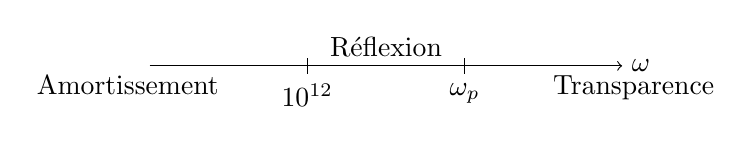
\begin{tikzpicture}
		\draw (0,0) -- node[below left]{Amortissement} (2,0) -- node[above]{Réflexion} (4,0);
		\draw[->] (4,0) -- node[below right]{Transparence} (6,0) node[right]{\( \omega \)};
		\draw (2,-.1) node[below]{\( 10^{12} \)} -- ++(0,.2);
		\draw (4,-.1) node[below]{\( \omega_p \)} -- ++(0,.2);
	\end{tikzpicture}
\end{center}



\end{document}
